% MAURI-003 TODO -- methodology expansion plan.
% Purpose: expand this chapter later from a method description into a more
% complete modelling-methodology chapter, without duplicating the validation
% chapter.
% Source base already cited here: Bonatte2026DMEM. Also check the
% HiStrA/DMEM manual and related DMEM articles before converting these notes
% into final prose.
% Suggested structure for the later expansion:
% - add a short subsection explaining the modelling hierarchy: macro-element,
%   zero-thickness interfaces, orthogonal links, sliding links, and diagonal
%   shear link;
% - state the material classes used in the thesis models, especially masonry,
%   backfill/soil, weak interfaces, and soil--foundation support;
% - tabulate the mechanical parameters required by each material/link type
%   and identify which parameters come from experiments, literature, or
%   calibration;
% - separate constitutive assumptions from numerical implementation details;
% - add a validation roadmap that points forward to the DMEM validation chapter
%   and clarifies which behaviours are checked by each benchmark.

% I have to \cite{Falco2026} regarding the Poisson effect. Also, he has a nice Fig 2 that discribe "Non-conforming discretization"
% I also must explain the tolerance values of convergence.

\typeout{NT FILE dmem_strategy.tex}

\chapter{Discrete Macro-Element Modelling Strategy for Masonry Arch Bridges}
\label{cha:dmem-strategy}

The structural assessment framework adopted in this thesis requires a numerical model able to describe the nonlinear behaviour of \gls{MAB}s while remaining efficient enough for repeated simulations. This chapter presents the \gls{DMEM} strategy used for that purpose. The material is based on the modelling developments validated in \cite{Bonatte2026DMEM}, but is rewritten here as thesis methodology and connected to the broader objective of risk-informed and resilience-oriented assessment.

\section{Role of the Macro-Element}
\label{sec:dmem-macro-element}

In the \gls{DMEM}, the bridge is discretised into macro-portions whose mechanical response is represented by equivalent macro-elements. This differs from a classical \gls{DEM} approach, where each element is usually idealised as a rigid block. In the \gls{DMEM}, each macro-element retains shear deformability and interacts with adjacent macro-elements through zero-thickness nonlinear interfaces. The axial and flexural response is therefore concentrated at the interfaces, whereas the in-plane shear deformation is governed by internal shear degrees of freedom and calibrated links.

This modelling philosophy is particularly suitable for \gls{MAB}s. The main bridge components, namely arch barrels, piers, abutments, spandrel walls, and backfill, can be represented with a reduced number of deformable macro-elements. The model can still reproduce flexural cracking, shear-diagonal failure, sliding, out-of-plane flexural response, and torsional effects, but avoids the very large number of degrees of freedom usually required by detailed mesoscale \gls{FEM} or block-by-block \gls{DEM} models.

\begin{figure}[htbp]
\centering
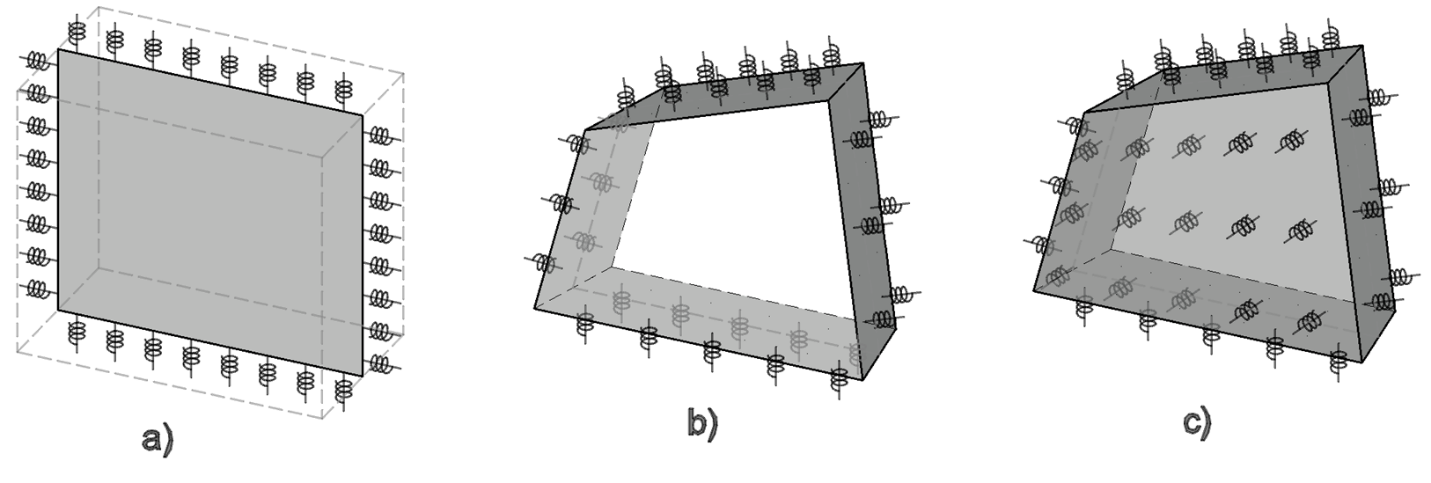
\includegraphics[width=0.95\linewidth]{./Figures/image1.png}
\caption{Evolution of the \gls{DMEM} approach from plane macro-elements to irregular spatial elements with interfaces on all faces \cite{Bonatte2026DMEM}.}
\label{fig:dmem-evolution}
\end{figure}

The macro-element adopted in this thesis extends previous spatial \gls{DMEM} formulations by introducing interaction surfaces on all six faces of the hexahedral element, as schematically illustrated in \Cref{fig:dmem-evolution}. This feature is essential for masonry arch bridge modelling because load transfer does not occur only through lateral contacts. In massive bridge components and backfill volumes, interaction through top and bottom faces is also required to reproduce load diffusion, passive resistance, and three-dimensional confinement effects.

\section{Kinematics and Zero-Thickness Interfaces}
\label{sec:dmem-interfaces}

Each three-dimensional macro-element is governed by rigid-body degrees of freedom and an additional shear deformability parameter. The rigid-body part describes translations and rotations, while the deformable part allows the element to reproduce shear distortion without requiring a fine continuum mesh. The relative displacement between two adjacent elements is evaluated at the corresponding interface and is then assigned to a set of nonlinear links.

\begin{figure}[htbp]
\centering
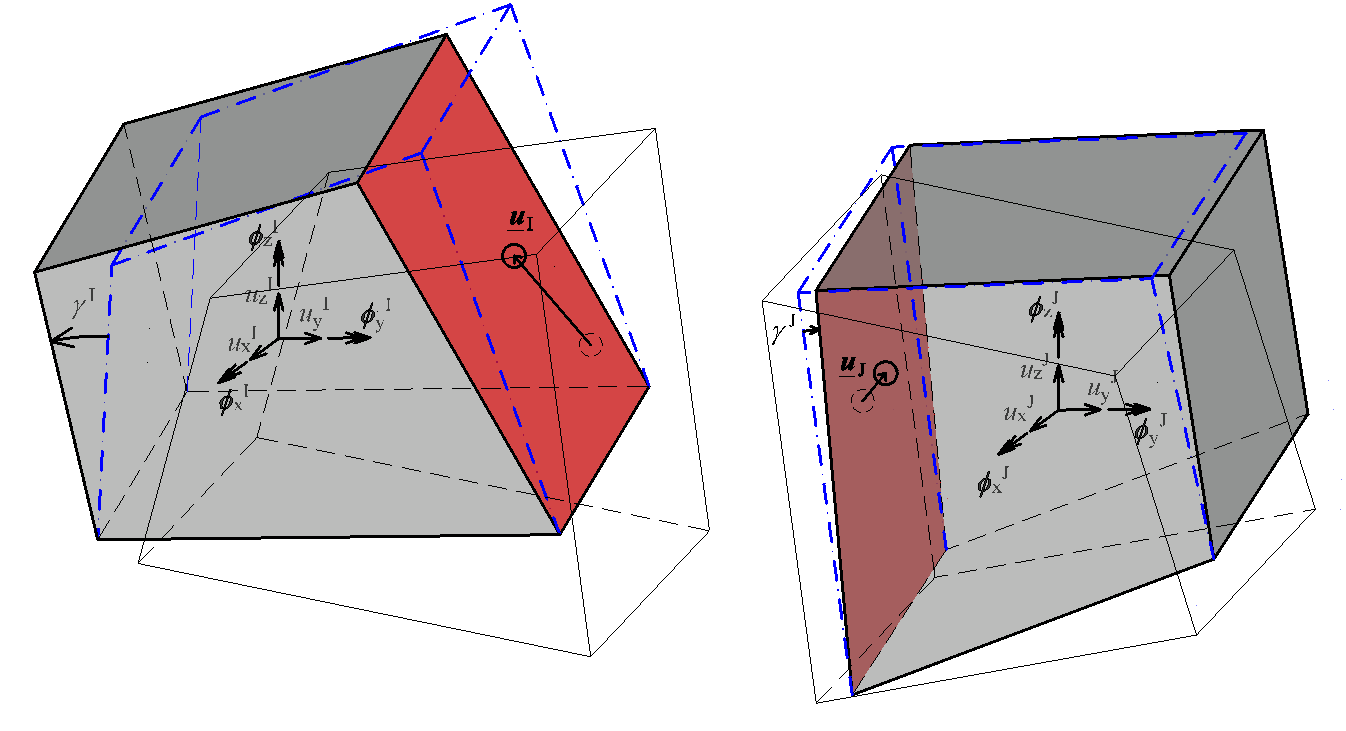
\includegraphics[width=0.75\linewidth]{./Figures/image2.png}
\caption{Kinematics of contiguous macro-elements and interface deformation in the \gls{DMEM} formulation \cite{Bonatte2026DMEM}.}
\label{fig:dmem-kinematics}
\end{figure}

The use of zero-thickness interfaces is central to the method. These interfaces are not physical gaps; rather, they are mechanical devices that concentrate the membrane, flexural, and sliding response between adjacent macro-elements. Controlled penetration between adjacent elements is permitted because axial and flexural behaviours are intentionally embedded at the interfaces. This is a modelling assumption rather than an overlap of real material, and it allows the interface links to reproduce the stiffness and strength of the finite material portions represented by the adjacent macro-elements.

The interfaces are calibrated by a fibre strategy. Each orthogonal link represents a strip of material associated with an influence area, and the link stiffness and strength are obtained from the mechanical properties of that material strip. The extension of the macro-element to six faces required the calibration to be generalised to the three principal directions of the hexahedral element, rather than only to the lateral surfaces used in previous shell-like macro-elements.

\section{Orthogonal Links}
\label{sec:dmem-orthogonal-links}

Orthogonal links reproduce membrane and flexural deformations normal to each interface. They are distributed over the zero-thickness interface and calibrated so that the assembly reproduces the elastic and inelastic response of the corresponding macro-portion of masonry or backfill. In masonry components, these links are assigned the elastic modulus, compressive strength, tensile strength, and fracture energy required to describe cracking, crushing, and post-elastic response.

\begin{figure}[htbp]
\centering
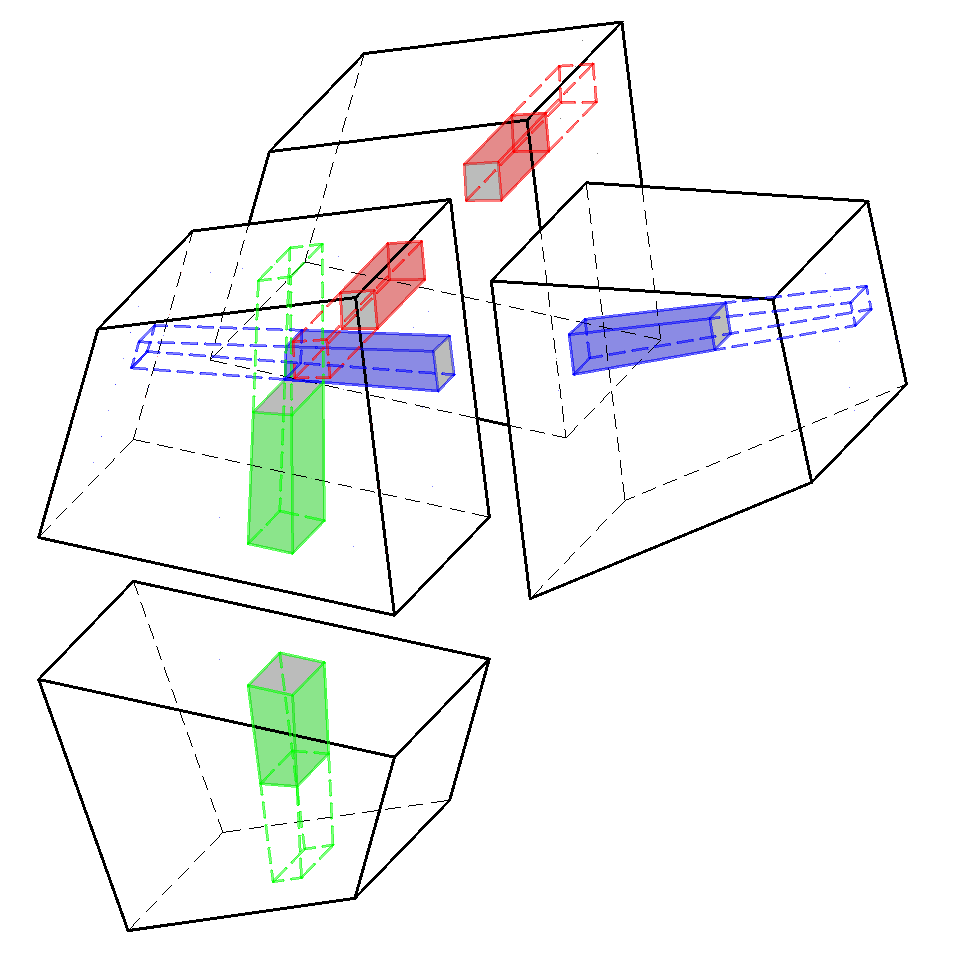
\includegraphics[width=0.65\linewidth]{./Figures/image3.png}
\caption{Fibre calibration concept for the transversal interface links in the spatial \gls{DMEM} element \cite{Bonatte2026DMEM}.}
\label{fig:dmem-fibre-calibration}
\end{figure}

The post-elastic behaviour of orthogonal links can be defined through different constitutive laws, including linear hardening, linear softening, exponential softening, and parabolic laws. In the bridge models considered in this thesis, linear softening is adopted for tensile and compressive flexural failure, with fracture energy controlling the post-peak response. This choice provides a direct way to dissipate energy during crack propagation and avoids an unrealistically brittle global response.

\section{Shear-Sliding Links}
\label{sec:dmem-sliding-links}

Shear-sliding links govern the tangential interaction between adjacent macro-elements. In spatial models, three nonlinear sliding links are required to reproduce the relevant failure mechanisms. One link controls the main in-plane sliding behaviour, while two additional links describe out-of-plane sliding and the associated torsional response around the axis normal to the interface.

\begin{figure}[htbp]
\centering
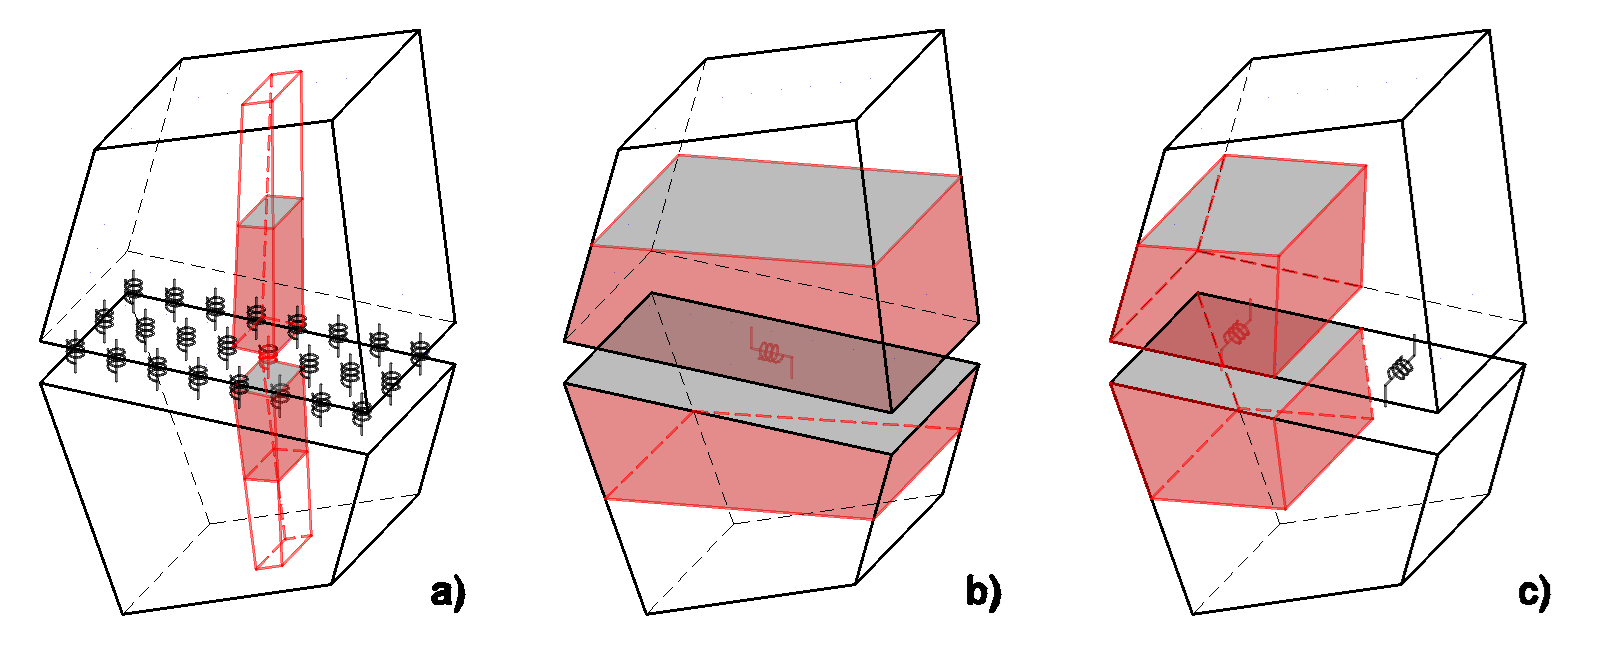
\includegraphics[width=0.65\linewidth]{./Figures/image5.png}
\caption{Interface link scheme used to represent orthogonal, in-plane sliding, and out-of-plane sliding mechanisms \cite{Bonatte2026DMEM}.}
\label{fig:dmem-interface-links}
\end{figure}

The shear-sliding links are governed by an elasto-plastic law with a Mohr--Coulomb yield domain. Their resistance depends on the current normal force and on the interface friction and cohesion. This is important for masonry arch bridges because sliding mechanisms may develop at mortar joints, between arch rings, at masonry--backfill contacts, or along deliberately weakened interfaces representing defects. In the case of ring separation, the interface between arch rings is assigned reduced mechanical properties and a friction coefficient compatible with the defective contact identified in the experimental campaign.

\section{Diagonal Link}
\label{sec:dmem-diagonal-link}

The diagonal link represents the in-plane diagonal shear behaviour of the macro-element. Its deformation is directly related to the shear degree of freedom of the articulated element. In the elastic range, the stiffness of the diagonal link is obtained by imposing energy equivalence between the macro-element and a geometrically consistent continuous reference model. The yielding force is then computed from the selected shear criterion and the current stress state of the element.

\begin{figure}[htbp]
\centering
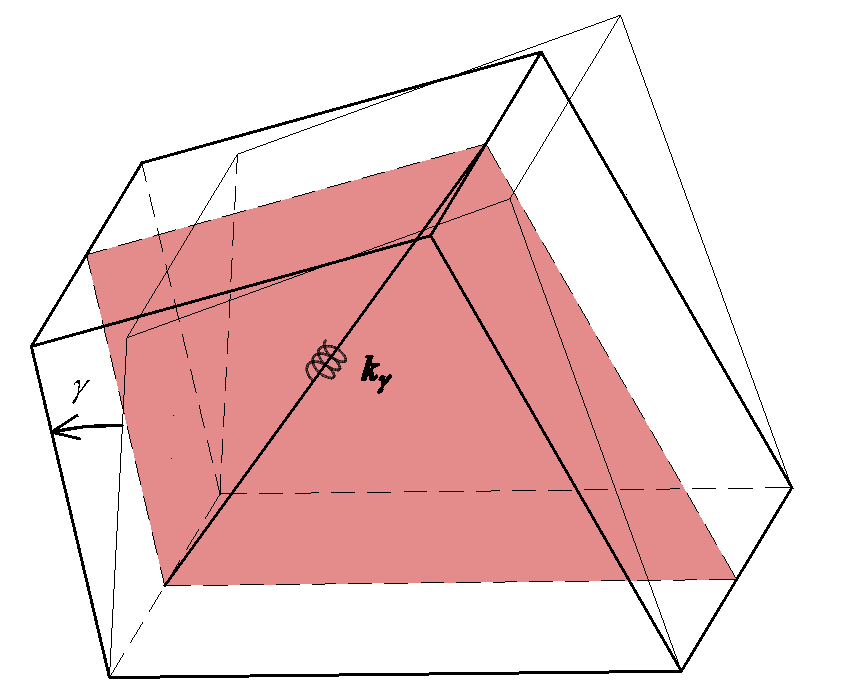
\includegraphics[width=0.55\linewidth]{./Figures/image4.png}
\caption{Diagonal shear link used to introduce in-plane shear deformability in the macro-element \cite{Bonatte2026DMEM}.}
\label{fig:dmem-diagonal-link}
\end{figure}

The diagonal shear mechanism may be governed by Mohr--Coulomb or Turnsek--Cacovic type criteria, depending on the material and calibration assumptions. In the present application, the Mohr--Coulomb criterion is used consistently with the interface sliding laws, allowing the influence of compression level, cohesion, and friction to be accounted for in a compact form.

\section{Three-Dimensional Hexahedral Macro-Element}
\label{sec:dmem-hexahedral}

The hexahedral macro-element introduced for \gls{MAB}s is the key development that makes the method suitable for bridge applications. Earlier \gls{DMEM} models were effective for walls, arches, and shell-like curved structures, but bridge assessment requires interaction through all spatial directions. Arch barrels interact with backfill through their extrados, backfill distributes loads vertically and laterally, spandrel walls provide transverse restraint, and piers and abutments transmit forces through three-dimensional contact surfaces.

The adopted element therefore includes interfaces on the four lateral faces and on the top and bottom faces. This allows the same formulation to be used for masonry and non-masonry components, including the backfill. It also allows strip models and full three-dimensional models to be built within a consistent numerical framework. Strip models are efficient for bridges with detached spandrel walls and uniform line loads, whereas full three-dimensional models are required when attached spandrel walls, eccentric loading, transverse effects, or strong spatial interaction must be represented.

\section{Modelling of Masonry and Backfill}
\label{sec:dmem-materials}

Masonry is treated as an equivalent orthotropic or homogenised material at the macro-element scale. The adopted input parameters include the unit weight, Young's modulus, compressive strength, tensile strength, cohesion, friction coefficient, and fracture energies in tension and compression. The zero-thickness interface links use these parameters to reproduce flexural cracking, crushing, sliding, and diagonal shear mechanisms.

The backfill is also represented by macro-elements. This is a deliberate modelling choice because the backfill has two primary structural roles in masonry arch bridges. First, it diffuses the applied vertical loads before they reach the arch barrel. Second, it provides weight and passive resistance when the arch deforms upwards near the extrados. By modelling the backfill explicitly, the method avoids relying only on empirical load-dispersion rules or calibrated passive pressure springs.

The current macro-element formulation does not include Poisson effects. This simplification is acceptable for the validation cases considered here because the main role of the backfill is load diffusion and passive resistance. Nevertheless, it limits the direct representation of confinement and dilatancy effects, especially where spandrel walls laterally restrain the fill. A compressive strength must also be assigned to the backfill because the fibre calibration procedure requires compression and tension resistance parameters. In the validation models, a backfill compressive strength of 0.9 MPa is adopted to avoid artificial local crushing while preventing the fill from unrealistically dominating the load-bearing capacity.

\section{Spandrel Walls and Ring Separation}
\label{sec:dmem-spandrels-rings}

Two configurations of spandrel walls are considered in the validation strategy. In bridges with detached spandrel walls, the experimental specimens included a narrow gap between the inner face of the spandrel wall and the edge of the arch barrel. The wall did not act compositely with the arch barrel, but it still laterally confined the backfill. These cases can be efficiently modelled with a strip model when the loading is a uniformly distributed line load and the geometry is square or nearly square.

In bridges with attached spandrel walls, a full three-dimensional model is necessary. Multiple macro-elements are introduced across the bridge width so that the arch barrel, backfill, load patch, and spandrel walls can interact. This transverse discretisation is essential because attached spandrel walls reduce vertical displacements near the bridge edges and produce a non-uniform displacement profile across the arch width.

Ring separation is represented by weak frictional interfaces between arch rings. These interfaces allow the rings to slide and deform more independently, thereby reproducing the reduction of composite action observed in defective multi-ring arch barrels. This defect has a strong effect on load capacity and failure mechanism, as shown in the validation chapter.

\section{Nonlinear Analysis Strategy}
\label{sec:dmem-analysis-strategy}

The bridge models are analysed through nonlinear incremental static analysis. The vertical load is applied progressively and the equilibrium path is solved using an iterative Newton--Raphson procedure. Convergence is checked through an energy criterion based on the norm of the product between the residual unbalanced force vector and the displacement increment vector.

The load increment is controlled by an arc-length algorithm. This is important for tracing nonlinear equilibrium paths near peak load and in the post-peak range, where a simple force-control strategy may fail. The arc-length procedure regulates the step size and improves numerical robustness in the presence of cracking, sliding, and stiffness degradation.

The discretisation adopted in the validation models follows two principles. First, the macro-element size is generally kept below 30 cm to represent the geometry and expected crack patterns with sufficient detail. Second, the spacing of interface springs is kept below approximately 10 cm. Most models use three rows of orthogonal interface springs, with local refinements introduced where ring separation, localised damage, or transverse effects require a more detailed representation. Sensitivity checks reported in the validation chapter show that further refinement produces only marginal changes in the global response for the analysed bridges, supporting the computational efficiency of the adopted strategy.

% \section{Relevance for the Thesis Framework}
% P-Delta is not available in the commercial software, only in the development one.
% Should I show the comparition?
% Actually, the PdeltaEffect is presented in the HXR file. The default value is "None", but may be changed to "EachStep" and "EachIteration".
% I have to compare the results to see the influence of the PdeltaEffect in the final output!
% I did a first comparison. What I observed is that the without the P Delta, the self-weight reduces 10% and then it comes back. With P delta, this variation is lower.
% Another observation is that P delta gave lower values than without it.

\section{Relevance for the Thesis Framework}
\label{sec:dmem-framework-relevance}

The \gls{DMEM} strategy is adopted in this thesis because it provides the type of structural response required by the subsequent risk and resilience framework. It is sufficiently detailed to produce load-displacement curves, collapse mechanisms, displacement capacity, and damage information, while being efficient enough for parametric analysis and future probabilistic workflows. The following chapter validates this strategy against experimental and numerical benchmarks before it is used as a core modelling component of the PhD research.
